\section{Archivos de Lanzamiento}
Anteriormente vimos cómo ejecutar un nodo. Pero en un proyecto grande de ROS, necesitaremos lanzar muchos más nodos. Necesitamos una forma de ejecutar muchos nodos con un sólo comando. Para esos sirven los archivos de lanzamiento o launch files. 

Un launch file permite realizar varias configuraciones para el ambiente y ejecutar multiples nodos.

Para poder usar launch files, realizar los siguientes pasos:
\begin{enumerate}
    \item Dentro del archivo \texttt{package.xml} del paquete, agregar la siguiente línea dentro de las etiquetas \texttt{<package>}:
    
\begin{center}
  \begin{Verbatim}[gobble=4]
    <exec_depend> ros2launch </exec_depend>
  \end{Verbatim}
\end{center}

\begin{figure}[H] 
  \centering    
  \makebox[\textwidth][c]{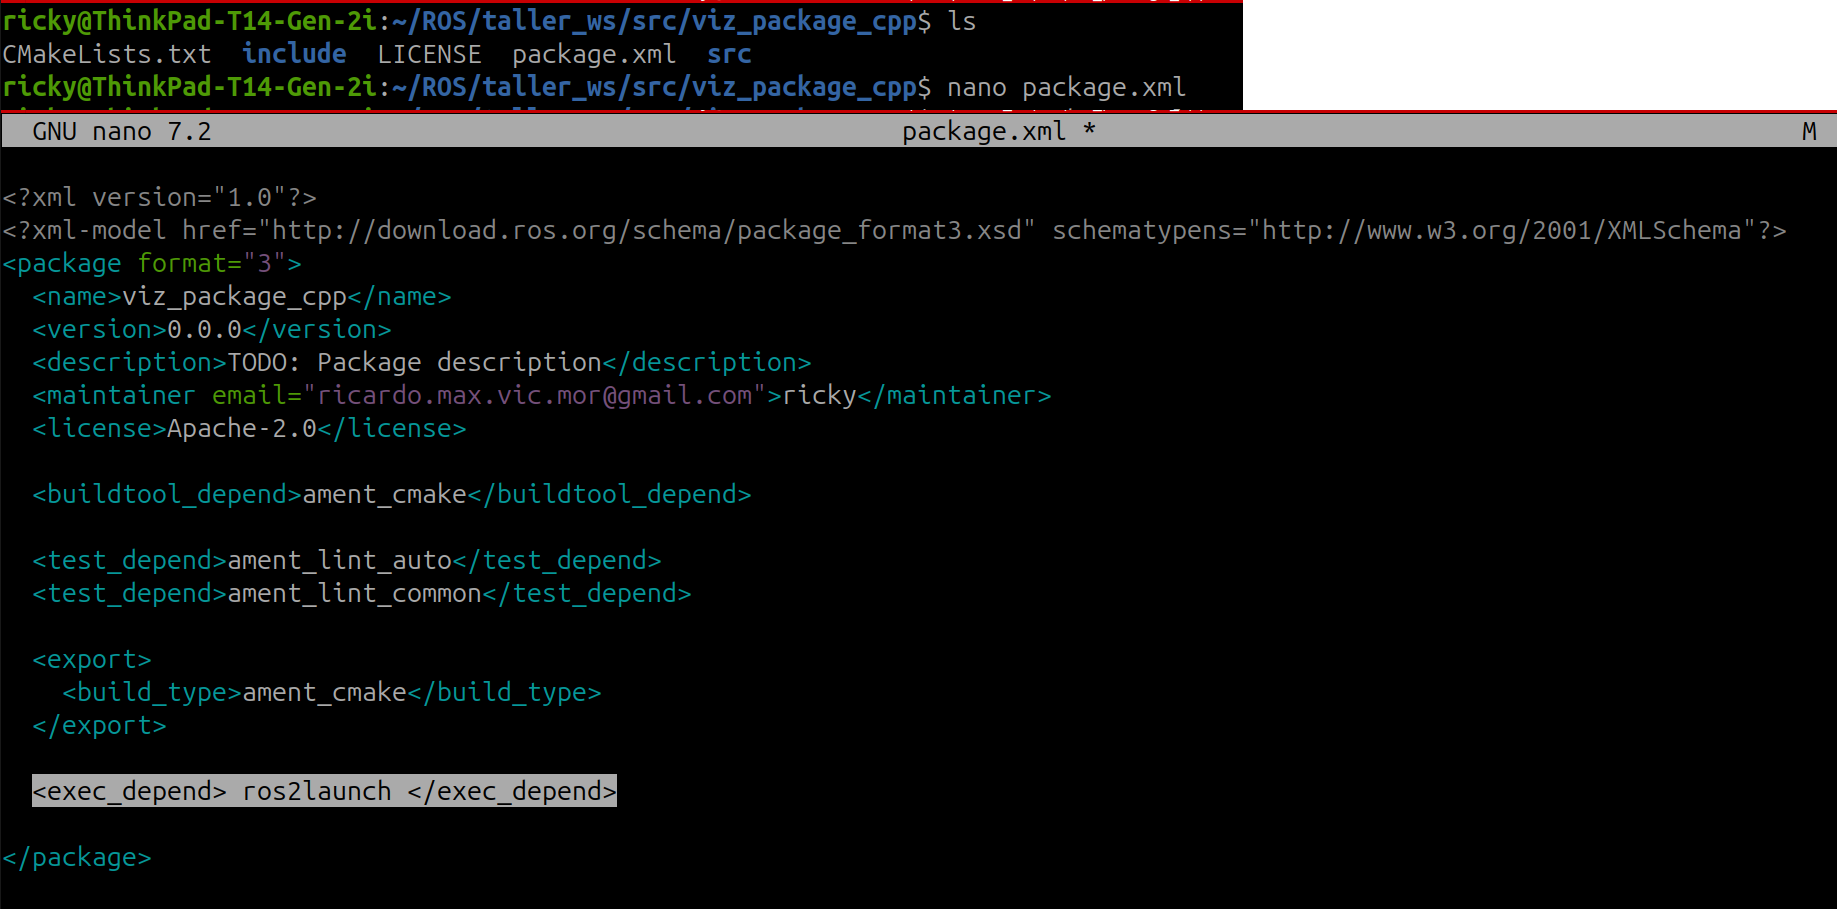
\includegraphics[width=1.4\textwidth]{imagenes/package.png}}
  \caption{Edición de package.xml para habilitar launch files.}
  \label{fig:mi_imagen}
\end{figure}

\item Crear una carpeta \texttt{launch} dentro del paquete.

\begin{figure}[H] 
  \centering    
  \makebox[\textwidth][c]{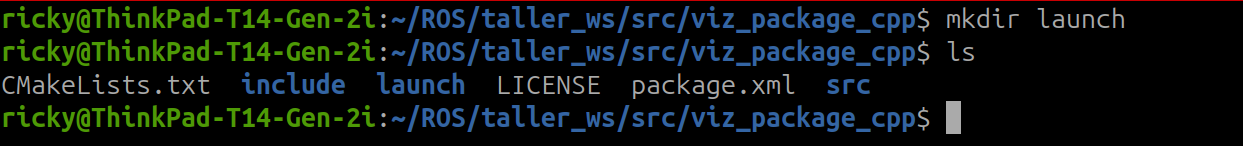
\includegraphics[width=1.4\textwidth]{imagenes/4.png}}
  \caption{Creación carpeta launch.}
  \label{fig:mi_imagen}
\end{figure}

\item Dentro de la carpeta \texttt{launch}, creamos un archivo de lanzamiento\\\texttt{viz\_launch.py} con el contenido que se ve en la imagen siguiente.

\begin{figure}[H] 
    \centering    
    \makebox[\textwidth][c]{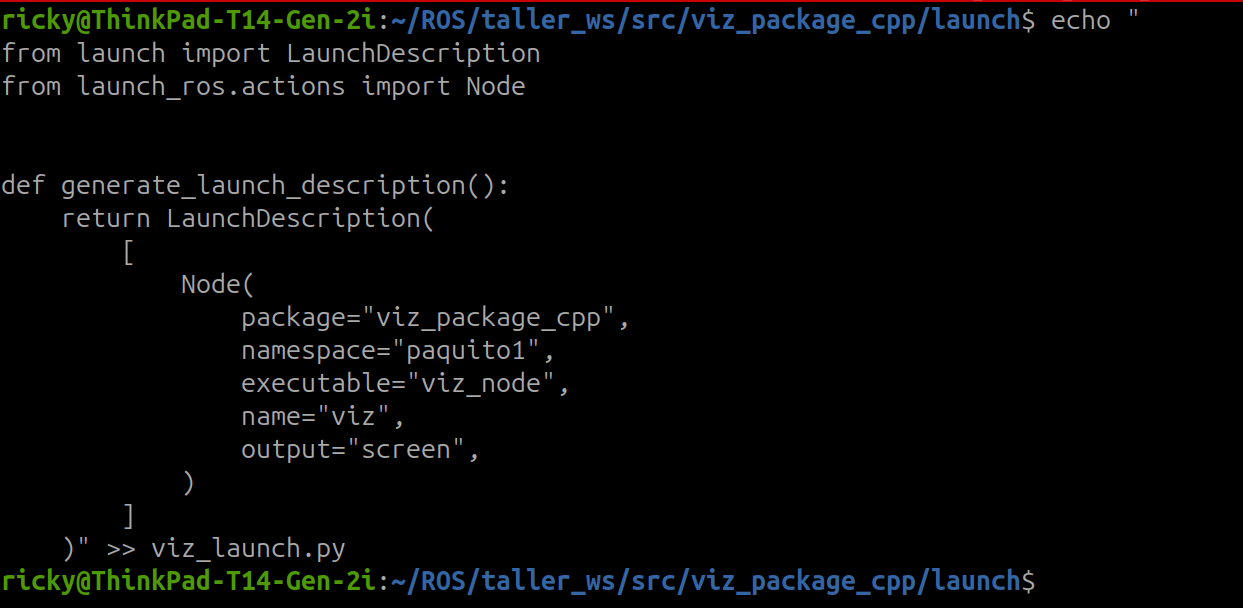
\includegraphics[width=1.4\textwidth]{imagenes/vizlaunch.png}}
    \caption{Creación carpeta launch.}
    \label{fig:mi_imagen}
\end{figure}
\item Volvemos a compilar.
\end{enumerate}




Con los pasos anteriores, ya podemos hacer uso de nuestro archivo de lanzamiento \texttt{viz\_launch.py}, el cual lanza el nodo \texttt{viz\_node}. Para lanzar el launch file nos ubicamos en la carpeta \texttt{launch} del paquete, y hacemos:

\begin{center}
  \begin{Verbatim}[gobble=4]
    ros2 launch <nombre archivo lanzamiento>
\end{Verbatim}
\end{center}

\begin{figure}[H] 
    \centering    
    \makebox[\textwidth][c]{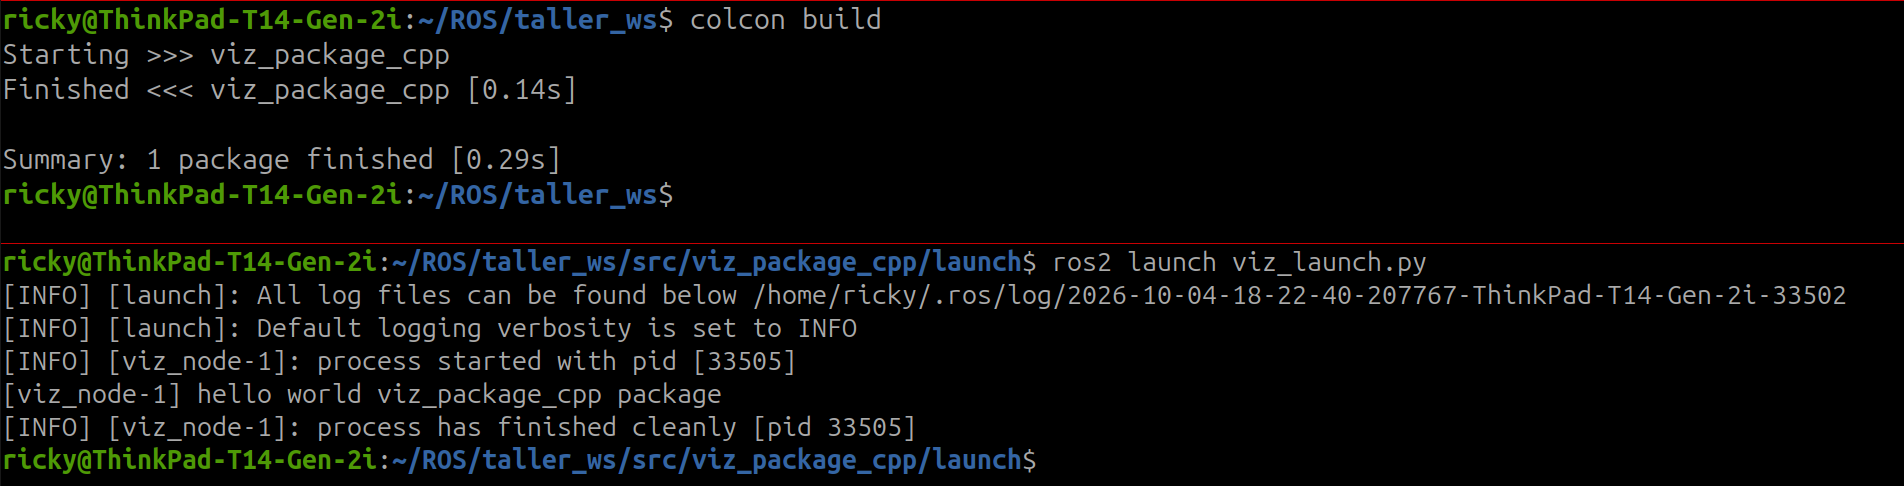
\includegraphics[width=1.4\textwidth]{imagenes/lanzandomix.png}}
    \caption{Lanzando nuestro primer launch file.}
    \label{fig:mi_imagen}
\end{figure}


Ahora, para poder lanzar el launch file sin tener que ubicarnos en la carpeta launch, hacemos lo siguiente:
\begin{enumerate}
  \item Abrir el archivo \texttt{CMakeLists.txt} del paquete, y agregar lo siguiente:
  \begin{center}
    \begin{Verbatim}[gobble=4]
      install(DIRECTORY
      launch
      DESTINATION share/${PROJECT_NAME}
      )
    \end{Verbatim}
  \end{center}

  \begin{figure}[H] 
      \centering    
      \makebox[\textwidth][c]{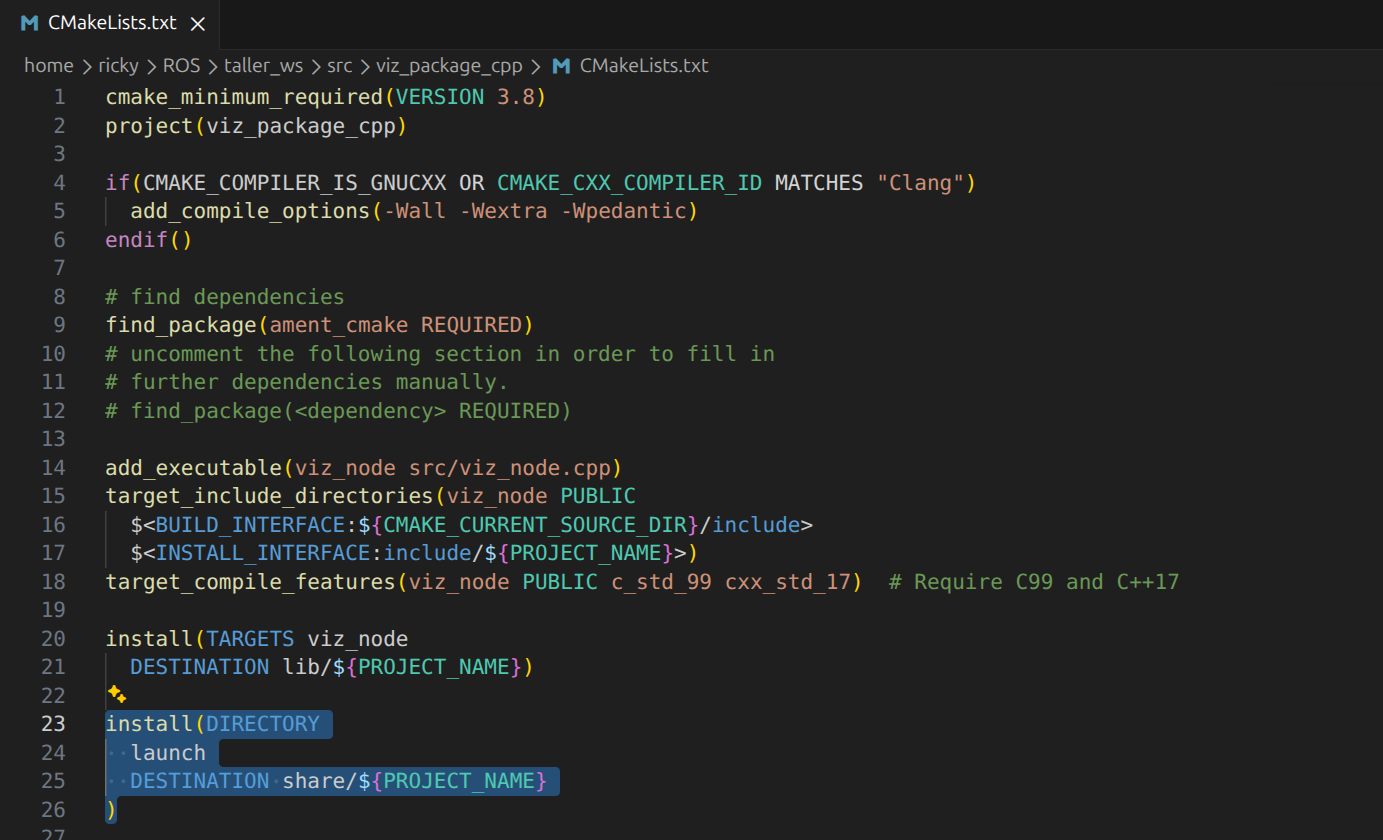
\includegraphics[width=1.4\textwidth]{imagenes/cmake.png}}
      \caption{Editar \texttt{CMakeLists.txt} para que los archivos launch se guarden en la carpeta \texttt{share}.}
      \label{fig:mi_imagen}
  \end{figure}
  
  \item En una terminal y en el espacio de trabajo, compilar con \texttt{colcon build}.
  \item En otra terminal y en el espacio de trabajo, activar el overlay con \texttt{source install/local\_setup.bash} y lanzar el launch file con \texttt{ros2 launch viz\_package\_cpp viz\_launch.py}
  
  \begin{figure}[H] 
      \centering    
      \makebox[\textwidth][c]{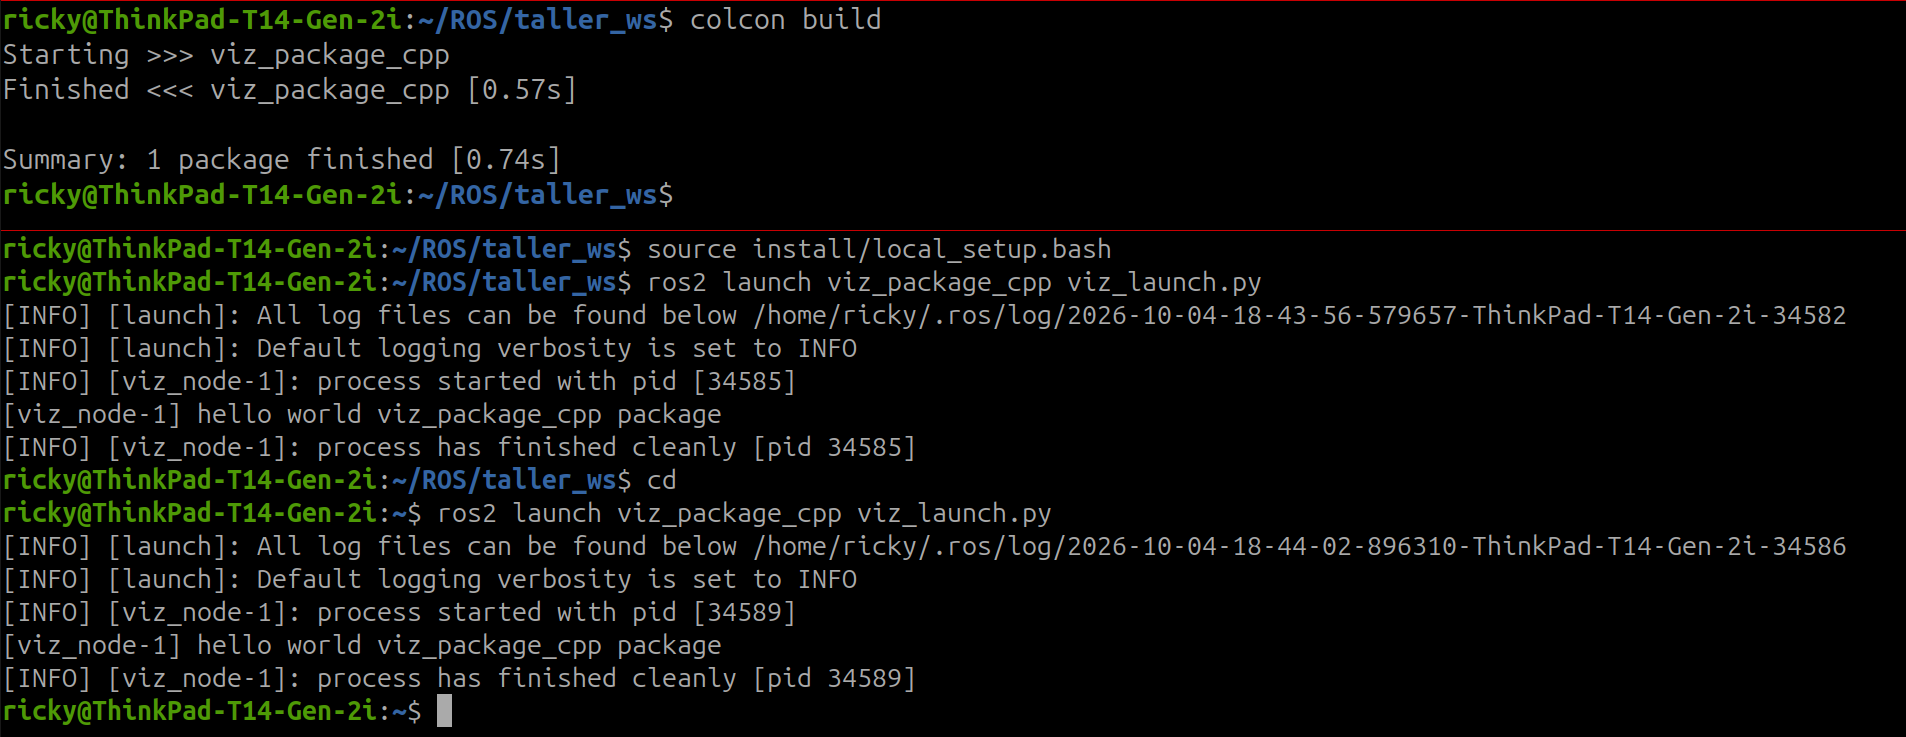
\includegraphics[width=1.4\textwidth]{imagenes/launchfinal.png}}
      \caption{Ahora se puede lanzar el launch file en cualquier ruta.}
      \label{fig:mi_imagen}
  \end{figure}

\end{enumerate}

